\section{Introduzione a UML}
\textbf{Unified Modeling Language} (UML) è un linguaggio standardizzato per il supporto alla descrizione e alla progettazione dei sistemi software. Sebbene sia tendenzialmente utilizzato in contesti orientati agli oggetti, è possibile usufruirne anche per descrivere sistemi hardware o comprendere il dominio operativo nel quale si lavora.\par
Presenta lo standard \textbf{Object Management Group} (OMG) e unifica in una singola collezione le varie notazioni pre-esistenti, integrandole e rendendole orientate agli oggetti. Si tratta di un linguaggio per la \textbf{modellazione} usato spesso in ambito lavorativo da analisti e progettisti software. Non è possibile usarlo per la programmazione. I tre utilizzi principali di UML riguardano: \begin{itemize}
	\item \textbf{Abbozzi}: Aiutano la comunicazione e la discussione, presentando solo le informazioni più importanti. Nella pratica sono usati tool come editor grafici o più direttamente una lavagna.
	\item \textbf{Progetti dettagliati}: Forniscono un modello completo da implementare mediante un modellatore UML, come Papyrus o Visual Paradigm.
	\item \textbf{Linguaggi di programmazione}: Meno comune dei due precedenti, è possibile usare dei tool appositi come UniMod per ottenere un modello eseguibile direttamente dalla composizione UML.
\end{itemize}
\noindent Esistono inoltre tre principali prospettive nell'utilizzo di UML: in primis, quella \textbf{concettuale}, che fornisce un punto di partenza per lo sviluppo con la rappresentazione dei concetti del dominio operativo; in secundis, quella di \textbf{specifica}, che vede descritte nel diagramma le interfacce del sistema senza dettagli implementativi; infine, la prospettiva di \textbf{implementazione} descrive gli elementi concreti del sistema software, come le classi e gli attori.\par
I sistemi in UML sono destritti tramite le \textbf{viste}, intese come un particolare aspetto del software da un punto di vista di un ruolo specifico. Lo scopo di un diagramma è la descrizione di una vista e il loro insieme compone il modello. Lo standard utilizzato in questo corso è UML 2.0, il quale contiene 13 tipi di diagrammi diversi divisi in due macro-categorie: \textbf{diagrammi strutturali}, i quali descrivono la struttura statica del sistema e \textbf{diagrammi comportamentali}, che rendono il comportamento dinamico.\par
UML è un linguaggio versatile; può essere utilizzato con qualsiasi processo nelle fasi di raccolta requisiti, design architetturale e delle componenti. Per esempio, nella prima fase è possibile usare un use case diagram per la descrizione dei requisiti funzionali del sistema da una vista dell'utente.
\begin{figure}[h]
	\centering
	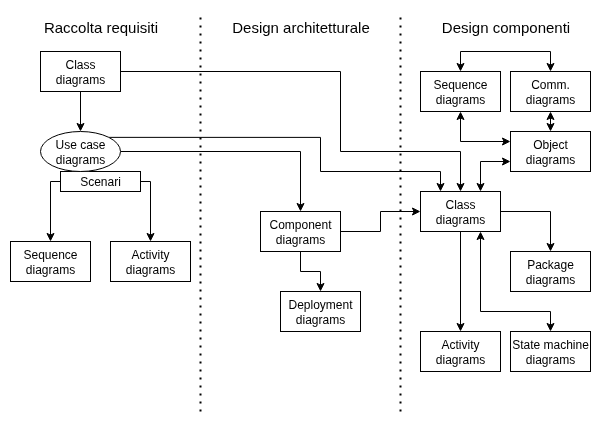
\includegraphics[width=1\linewidth]{Images/UML_diagrams_overview.png}
	\caption{Panoramica diagrammi UML 2.0}
\end{figure}

\noindent Non sempre è sufficiente l'implementazione dei diagrammi UML nel workflow; esistono due soluzioni principali per essere più esaustivi: \textbf{non usare} UML oppure l'\textbf{estensione} del diagramma tramite \textbf{profili}, andando a sacrificare lo standard. Per quest'ultima soluzione è possibile specificare particolari domini applicativi o tipi di applicazioni; un profilo è costituito principalmente da: \begin{itemize}
	\item \textbf{Stereotipi}: Elementi aggiuntivi ottenuti modificando quelli già esistenti.
	\item \textbf{Vincoli aggiuntivi}: Ulteriori restrizioni rispetto a quelle standard presenti in UML.
	\item \textbf{Informazioni semantiche aggiuntive}: Per dare ulteriori delucidazioni in merito agli elementi.
\end{itemize}
\noindent Quello di estendere i diagrammi rendendoli \textbf{illegali} è un compromesso utilizzato spesso in ambito lavorativo. Ciò fa capire quanto sia fondamentale la flessibilità ai contesti rispetto all'attenersi esclusivamente agli standard e ai manuali. Lo sviluppo software è un processo creativo. Divertiti.

%

\section{Class e Object Diagram}
I \textbf{diagrammi di classe} definiscono le classi e relativi attributi, operazioni e relazioni con altre entità, come associazioni, aggregazioni, composizioni, specializzazioni, generalizzazioni e dipendenze. Modellano quindi la parte strutturale (o statica) di un sistema software.\par
Il concetto di classe in UML è identico a quello presentato nel paradigma di orientamento agli oggetti; vengono rappresentare da un rettangolo diviso in più compartimenti, i quali contengono nome, attributi e operazioni rispettivamente. Per quanto riguarda gli \textbf{attributi} presentano la segnatura: \begin{center}
	visibilità nome: tipo [molteplicità] = default\{proprietà\}
\end{center}
\noindent Dove default è il valore base dell'attributo di un oggetto appena creato e proprietà definisce vincoli come sola lettura. Il nome è l'unica parte obbligatoria da indicare, mentre le altre sono facoltative. Presentano inoltre quattro simboli corrispondenti ai modificatori di accesso, validi anche per le operazioni, discusse più avanti: \begin{itemize}
	\item \textbf{Public}: +
	\item \textbf{Private}: -
	\item \textbf{Protected}: \#
	\item \textbf{Package private}: $\sim$
\end{itemize}
\noindent Anche la \textbf{molteplicità} è un dato che può presentare più valori e corrisponde a un quantitativo degli attributi, come per esempio le dimensioni di una lista concatenata. Il valore di \textbf{default} è 1 e indica che nel software esiste una sola classe di questa fattura. Alternativamente è possibile usare $0..1$ per dire \textbf{al più uno}, $0..*$ per \textbf{nessuno o numero imprecisato}, $1..*$ per \textbf{almeno uno}, oppure per generalizzare, usare $n,m$, definendo i loro valori. Le \textbf{operazioni} invece presentano la segnatura: \begin{center}
	visibilità nome(parametri): tipo-ritornato\{proprietà\}
\end{center}
\noindent 



\begin{comment}		
	La lista dei parametri contiene nome e tipo dei parametri, secondo la segnatura <direzione nome: tipo = default>.
	La direzione è intesa come input (in), output (out) o entrambi (inout). Il default è input. I getter/setter non sono inseriti, è scontato che ci siano.
	In UML esistono due operazioni:
	- query: ottengono un valore da un oggetto senza side effect
	- modificatori: modificano lo stato dell'oggetto su cui sono chiamate
	
	In UML esiste il concetto di data type che è diverso dagli oggetti. Non sono istanze, non hanno identità; le istanze sono valori in questo caso.
	Degli esempi sono le date o un valore monetario, che hanno senso esclusivamente con i valori. Si indicano specificandoli con lo stereotipo <<datatype>> sopra il nome del tipo.
	
	-- Associazioni
	Un'associazione è una relazione tra le classi. Un -> indica la direzione in cui deve essere letta l'associazione. éer esempio Persona -> automobile indica che la persona possiede l'auto. In alternativa si può indicare il ruolo di uno dei due estremi dell'associazione.
	Puoi indicare questa cosa anche con il verso di navigazione, che indica in quale direzione è possibile reperire le infrmazioni. Con questo, puoi aggiungere anche la molteplicità. È comodo e compatto.
	
	Attributi e associazioni sono due modi per rappresentare la stessa cosa. Per convenzione si usano:
	- attributi per tipi primitivi e datatype
	- Associazioni se sono tipati da classi
	
	--- Object diagram
	Diagramma che consente di rappresentare le istanze di una classe. Considera tutte le possibili combinazioni valide. Servono a chiarire i class diagram più complessi, spiegando anche la relazione tra classe e oggetti con l'operazione <<istanzia>>.
	Le operazioni e i campi static corrispondono esattamente ai metodi e i static types di java. Per indicare che un campo è statico, lo si sottolinea.
	
	- Associazioni riflessive: una classe che ha associazione con sé stessa (parrebbe la relazione ricorsiva dello schema ER)
	- Classi associative
	Talvolta alcune proprietà sono proprie dell'associazione piuttosto che delle classi coinvolte; quindi si aggiunge un rettangolo alla relaizione, al quale è possibile aggiungere attributi e operazioni.
	
	- Asociazioni bidirezionali
	Quando da le informazioni sono recepibili da ambo le direzioni, quindi da entrambe le due classi coinvolte. Non è una cosa implementabile con un singolo attributo e da implementare sono un attimo complesse.
	Nel settare dei valori ad una classe con relazione bidirezionale, così bisognerà fare con l'altra a cui è legato. C'è dunque un problema di sincronizzazione. Per esempio, se ho classi Man e Woman e da una parte setto Man come marito della woman, a sua volta dovrà settare woman come moglie di Man. Per spiegare questo comportamento si esplicita che sono sincronizzate e si aggiunge una nota che specifica il comportamento.
	
	-- Aggregazione
	Altra relazione di tipo strutturale. Si indica con una freccia simil-diamond: regione -<> nazione.
	Una regione è parte di una nazione. Si tratta di una sfaccettatura più importante guardando al livello concettuale, perché a livello software si implementa con un'associazione.
	
	-- Composizione
	Forma più rigorosa di aggregazione. Se il composto è distrutto, così seguiranno le sue parti. È indicato con la diamond-arrow riempita. Le classi aggregate non hanno senso da sole, difatti.
	
	-- Generalizzazione ed ereditarietà
	Per generalizzazione intendiamo che ogni istanza di una classe è anche della superclasse, mentre l'ereditarietà è un meccanismo con il quale elementi specializzati incorporano la struttura ed il comportamento di elementi più generali.
	
	Attenzione che le operazioni e i metodi UML non sono la stessa cosa. Le operazioni sono invocate su oggetti e sono la dichiarazione di una procedura o funzione, mentre un metodo è il CORPO di tale procedura o funzione, quindi la sua definizione.
	
	-- Dipendenze
	Si ha una dipendenza tra due classi se la modifica di una comporta un cambiamento a un'altra.
\end{comment}

%

\section{Interfacce}

\begin{comment}
	15-24-26 - softEng - Incompleto
	
	--- Interfacce
	Per interfaccia intendiamo l'insieme delle operazioni visibili all'esterno degli oggetti, istanze di quella classe.
	Si tratta di un'entità simile ad una classe, ma priva di implementazione, che sarà definita con sue istanze concrete che la implementano.
	Una o più classi possono fornire l'implementazione dell'interfaccia.
	
	Per esempio in un gestionale di banca, le classi Impiegato e Bancomato forniscono l'interfaccia cassiere.
	In essa sono dichiarate le operazioni di ritiro e deposito contante; esistono due modi per rappresentarlo in UML:
	- Relazione di implementazione, detta anche realizzazione: Si indica con una linea tratteggiata e una freccia verso l'interfaccia.
	- Lollipop: Si usa una pallina per rappresentare l'interfaccia esposta/fornita da una classe e un semicerchio per rappresentare l'interfaccia richiesta.
	Si tratta quindi di una dipendenza. *Vedi immagine slide
	
	Le interfacce hanno senso di esistere per diminuire l'accoppiamento tra classi. Se più classi usano simili meccanismi, potrebbe essere corretto astrarli
	con un'interfaccia e farli definire concretamente dalle classi implementanti.
	
	Esistono delle regole di vincolo
\end{comment}

%

\section{Sequence e Communication Diagram}

\begin{comment}
	Lez11 - 16/04/26 softEng
	
	--- Sequence diagram e communication diagram
	
	I diagrammi di interazione descrivono la collaborazione di un gruppo di oggetti (scambio di messaggi).
	I messaggi possono presentarsi in tre modi:
	- sincroni: Il mittente si pone in attesa del risultato
	- Asincroni: Il mittente continua l'esecuzione; questi ultimi sono usati per rappresentare i processi concorrenti.
	- trovati: messaggi il cui partecipante che lo genera è omesso
	Per scambiare messaggi è necessario avere una relazione tra le classi.
	
	La notazione del sequence diagram presenta due attori principali detti partecipanti (sarebbero le classi) indicate con tre segnature possibili:
	[nomeClasse]: oggetto di nome nomeClasse non specificando il tipo
	[:nomeClasse]: istanza anonima di nomeClasse
	[s:nomeClasse]: istanza di nomeClasse chiamata s
	Messaggi sincroni inficati con frecce piene; la risposta con una freccia tratteggiata.
	Naturalmente coi messaggi è possibile specificarne anche i parametri, con segnatura [returnValie = message(params): returnType]
	
	I messaggi possono essere anche usati per la creazione di istanze; allora la risposta andrà dentro ad un oggetto creato. Per indicare invece che la vita di un oggetto termina, si usa una risposta che entra in una X. Un oggetto si può anche autodistruggere.
	Cicli e condizioni possono essere espressi con i frame di interazione; cornici per inquadrare una parte del diagramma. Il primo operatore è loop, il secondo invece è opt, per optional. Un terzo si chiama Alt, per alternate e si usa per gli if-else.
	Naturalmente è possibile annidare i frame, sebbene faccia schifo a vedersi.
	Ref è invece usato per semplificare i sequence diagram; indica una reference ad un metodo specifico. Al posto di indicare l'intero diagramma coi messaggi, si usa il nome accerchiato dal frame ref.
	L'ultimo operatore è par, sta per parallel e indica metodi eseguiti concorrentemente. Naturalmente non ha senso accerchiare un solo metodo con par.
	
	I SD sono un buon mezzo per visualizzare l'interazione tra oggetti astrattamente, non la logica di controllo. Rendono chiare le chiamate e le relazioni tra le classi. Sconsigliato usare i frame di interazione; per la logica di controllo usare pseudocodice.
	Normalmente gli SD sono usati a due livelli differenti: a livello di requisiti per spiegare gli use case e il funzionamento astratto, e a livello di design, per descrivere più facilmente le relazioni tra le classi e il modo in cui interagiscono.
	Un diagramma di sequenza di sistema illustra invece gli eventi di I/O del sistema relativi ad uno scenario o più di uno use case. Hai praticamente lo use case ed il flusso dei messaggi è descritto tramite SD.
	
	--- Diagrammi di interazione
	Simile ai sequence diagram, condivide la sintassi, ma si rappresentano i messaggi come etichette degli archi con una direzione. Semplifica la struttura del diagramma rispetto a prima.
	
	--- Esercizio (ordine)
	Supponiamo di avere un ordine di acquisto; ci serve un'operazione per calcolare l'importo totale scontato con o.calcolaPrezzo().
	Per farlo l'ordine deve determinare l'importo di tutti i suoi elementi di linea [Quantità*prezzoUnitario]; dopo aver calcolato il totale l'ordine deve calcolare uno sconto globale che dipende dal cliente e scalarlo.
	
	Dunque o.calcolaPrezzo = totale-sconto
\end{comment}

%

\section{State Machine Diagram}

\begin{comment}
	Lez13 - 23-04-26 softEng
	
	# Prossima lezione il 6 maggio
	
	--- State machine diagrams
	Diagrammi che descrivono il comportamento di un componente, in termini di variazione del suo stato interno quando riceve un input di qualche tipo. Modello FSM, in pratica. Uno stato rappresenta una situazione nella vita di un oggetto durante la quale sono soddisfatte determinate condizioni e possono essere eseguite delle attività. Si cambia stato in base agli input ricevuti dagli attori.
	Si rappresenta come una FSM (ma dai?) e sugli archi stanno descritti eventi e input.
	Una FSM è sempre associata a un'entita e ne descrive il relativo comportamento. Riceve eventi che sono salvati su una coda ed estratti uno alla volta; la semantica è di tipo run-to-completion, quindi un evento è estratto solo dopo che è stato estratto il precedente.
	Inoltre, se ci sono più transazioni eseguibili in un dato momento (non determinismo se due transizioni dallo stesso stato con stesso evento e due condizioni diverse sono entrambe vere) ne viene eseguita solo una.
	Pallino nero è stato iniziale, nodi sono gli altri stati, archi son le transizioni. Un pallino nero accerchiato è lo stato finale e indica che l'esecuzione è terminata. Possono essercene più di uno.
	
	Le transizioni specificano come si passa tra gli stati. Specifica evento (trigger che attiva il passaggio), guardia (condizione che se vera permette il passaggio di stato) e attività (una o più azioni che sono compiute prima di cambiare stato). Transizione avviene come risposta a un evento. Eventi guardie e attività sono opzionali.
	
	Possiamo associare le FSM a una classe o un singolo oggetto per la durata del suo ciclo di vita.
	
	Ci sono più tipi di evento. Il primo è la ricezione di un messaggio, ma può esserci anche un evento di cambiamento (quando condizione passa da falsa a vero) o un evento temporale (si verifica dopo un tempo t o a una data precisa); si indica con when(condizione) nell'arco.
	Uno stato può reagire ad eventi e compiere attività anche senza una transizione ad uno stato diverso. Si possono mostrare nel secondo slot e seguono la sintassi delle transizioni. In particolare, entry ed exit sono attività speciali che si attivano ogni volta che si entera/escher dallo stato.
	Esiste anche do-activity che è eseguita mentre l'oggetto è nello stato. Può durare per un intervallo di tempo ed essere interrotta da altri eventi.
	
	Uno stato può essere semplice o composito. Quest'ultima forma consente di suddividere la complessità del modello. Nel senso, hai il macro-stato e una fsm interna. Si usa un'icona per rappresentare uno stato composito il cui comportamento interno non è mostrato.
	Possibile indicare concorrenza negli stati compositi aggiungendo slot alla macro-fsm.
	
	Entry ed exit points si indicano con cerchi bianchi e cerchi bianchi con una X all'interno rispettivamente.
	
	Quando è corretto usare le FSM? Per entità con una logica interna complessa.
	
	State machine si implementa in tre modi: switch case, con un design pattern state (ogni stato è una classe, si usa il polimorfismo per variare il comportamento) o delle STT con un tool che traduce da linguaggio apposito.
\end{comment}
